\typeout{(body.tex)}

\begin{frame}
    \titlepage
\end{frame}

%\begin{comment}
\begin{frame}{last time}
    \begin{itemize}
    \item classes
        \begin{itemize}
        \item declarations in {\tt .h} file
        \item {\tt ClassName::method}
        \item {\tt class ... \{...\}\myemph{;}}
        \item {\tt const}, {\tt static}
        \end{itemize}
    \item objects --- values, not references
        \begin{itemize}
        \item {\tt return Foo(1)} --- {\tt Foo(1)} is temporary Foo object
        \item {\tt x = y} --- copy {\tt x} into {\tt y}
        \end{itemize}
    \item the preprocessor --- {\tt \#define}, {\tt \#include}, etc.
    \item started pointers
    \end{itemize}
\end{frame}
\end{comment}

\begin{comment}
\begin{frame}{last time}
    \begin{itemize}
    \item pointers
        \begin{itemize}
        \item memory --- array of bytes
        \item pointers --- indices into array --- addresses
        \item {\tt T *} --- pointer to T type
        \item {\tt *somePointer} --- use thing at address `pointed to'
        \item {\tt \&someVariable} --- address of someVariable
            \begin{itemize}
            \item AKA ``pointer to'' someVariable
            \end{itemize}
        \end{itemize}
    \item started {\tt new}/{\tt delete}
    \end{itemize}
\end{frame}
\end{comment}

\begin{comment}
\begin{frame}[fragile,label=lastTime]{last time}
\lstset{language=C++,style=small}
    \begin{itemize}
    \item arrays in C++
        \begin{itemize}
        \item \lstinline|int foo[100];|
        \item \lstinline|int *foo = new int[100]; ... delete[] foo;|
        \item \lstinline|foo[42]|
        \end{itemize}
    \item references
        \begin{itemize}
        \item \lstinline|int &refToX = x;|
        \item \lstinline|refToX = valueToAssignToX;|
        \item \lstinline|funcNeedingInt(refToX);|
        \item automatically dereferenced pointers
        \end{itemize}
    \item references as function arguments/pass (started)
    \end{itemize}
\end{frame}

\begin{frame}{SDAC note-taking assistence}
    \begin{itemize}
    \item Student Disability Access Center website ---
        \begin{itemize}
        \item \url{https://studenthealth.virginia.edu/sdac}
        \item ``Notetaker Application'' link
        \end{itemize}
    \end{itemize}
\end{frame}
\end{comment}

\begin{frame}[fragile,label=lastTime]{last time}
\lstset{language=C++,style=small}
    \begin{itemize}
    \item references to const
    \item default methods and destructors
        \begin{itemize}
            \item \lstinline|Foo::Foo()| --- default constructor
            \item \lstinline|Foo::Foo(const Foo& other)| --- copy constructor
            \item \lstinline|Foo::~Foo()| --- destructors
            \item \lstinline|Foo &Foo::operator=(const Foo& other)| --- assignment
        \end{itemize}
    \item overriding operators
        \begin{itemize}
            \item \lstinline|operator>>|, \lstinline|opreator<<| for \lstinline|cin|, \lstinline|cout|
            \item \lstinline|operator+|, \lstinline|operator+=| for \lstinline|string|
            \item \ldots
        \end{itemize}
    \item \lstinline|operator<<|, etc. as method or global function
    \end{itemize}
\end{frame}


\section{priority queues}

\subsection{motivation}

\begin{frame}{priority queues: motivation}
\begin{itemize}
\item dynamically changing list of events with dates
    \begin{itemize}
    \item want to find next event quickly
    \end{itemize}
\item list of running programs, some more important (e.g. what user will notice being slow)
    \begin{itemize}
    \item choose most important to run first
    \item want to find most important quickly
    \end{itemize}
\item list of connections, some interactive (video call), some not (download)
    \begin{itemize}
    \item want quick way to choose which one to service
    \end{itemize}
\vspace{.5cm}
\item data structure: priority queue
\end{itemize}
\end{frame}


\subsection{the ADT}

\begin{frame}[fragile,label=prioADT]{priority queue ADT}
\lstset{language=C++}
\begin{itemize}
\item \lstinline|insert(priority, item)|
\item \lstinline|findMin()| --- return item with lowest (first) priority
\item \lstinline|deleteMin()| --- remove item with lowest (first) priority
\end{itemize}
\end{frame}

\begin{frame}[fragile,label=prioADTImpl]{priority queue implementations}
\lstset{language=C++}
\begin{tabular}{l|lll}
structure & insert & findMin & deleteMin \\
unsorted vector & $\Theta(1)$ (amortized) & $\Theta(n)$ & $\Theta(n)$ \\
unsorted linked list & $\Theta(1)$ & $\Theta(n)$ & $\Theta(n)$ \\
sorted vector & $\Theta(n)$ & $\Theta(1)$ & $\Theta(1)$ \\
sorted linked list & $\Theta(n)$ & $\Theta(1)$ & $\Theta(1)$ \\
balanced tree & $\Theta(\log n)$ & $\Theta(\log n)$ & $\Theta(\log n)$ \\
\myemph<2>{binary heap} & \myemph<2>{$\Theta(\log n)$} & \myemph<2>{$\Theta(1)$} & \myemph<2>{$\Theta(\log n)$} \\
\myemph<3>{Fibannoci heap} & \myemph<3>{amortized $\Theta(1)$} & \myemph<3>{$\Theta(1)$} & \myemph<3>{amortized $\Theta(\log n)$} \\
\end{tabular}
\end{frame}


\section{binary heaps}

\begin{frame}{binary heaps}
\begin{itemize}
\item binary heap is a binary tree
\item binary tree is \myemph{not a binary search tree}
\item structure: almost a perfect tree
\item ordering: parent $<$ child (everywhere in tree)
\end{itemize}
\end{frame} 


\subsection{recall: complete/perfect binary tree}

\usetikzlibrary{graphs,graphdrawing}
\usegdlibrary{trees}

\begin{frame}{perfect binary trees}
    \begin{tikzpicture}
\tikzset{
    >=Latex,
    mybst/.style={binary tree layout,level distance=10mm,sibling distance=15mm,nodes={draw,circle,inner sep=0.5mm,minimum width=.8cm,text=white}},
}
\begin{scope}[mybst]
\graph {
    [name=a] A[desired at={(0,0)}] -> {B -> {D, E}, C -> {F, G}} 
};
\end{scope}
\end{tikzpicture}
    \begin{itemize}
    \item a binary tree is \myemph{perfect} or \myemph{complete} if
        \begin{itemize}
        \item all leaves have same depth
        \item all nodes have zero children (leaf) or two children
        \end{itemize}
    \item \myemph{exactly} the trees that achieve $2^{h+1}-1$ nodes
    \end{itemize}
\end{frame}


\subsection{heap structure: almost complete tree}

\usetikzlibrary{graphs,graphdrawing}
\usegdlibrary{trees}

\begin{frame}{almost perfect/complete binary trees}
    \begin{tikzpicture}
\tikzset{
    >=Latex,
    mybst/.style={binary tree layout,level distance=5mm,sibling distance=5mm,nodes={draw,circle,inner sep=0.5mm,minimum width=.8cm,text=white}},
    missing/.style={alt=<1>{invisible},alt=<2>{dotted,draw=red},text=white, edge from parent/.style={draw=none}}
}
\begin{scope}[mybst]
\graph {
    [name=a] A[desired at={(0,0)}] -> {
        B -> {D -> {H, I}, E -> {J, Xb[missing,> missing]}},
        C -> {F ->[missing] {Xc[missing], Xd[missing]}, G ->[missing] {Xe[missing], Xf[missing]}}
    }
};
\end{scope}
\end{tikzpicture}
    \begin{itemize}
    \item heaps are \myemph{almost complete} trees
    \item only missing bottom-rightmost slots
    \end{itemize}
\end{frame}

\begin{frame}{almsot complete formally}
\begin{itemize}
\item single node tree is almost complete
\item otherwise: almost complete if either
    \begin{itemize}
    \item left child is complete with height $h$ and right child almost complete with height $h$; \textit{OR}
    \item left child is almost complete with height $h$ and right child is complete with height $h$
    \end{itemize}
\end{itemize}
\end{frame}


\subsection{almost complete trees as arrays}

\usetikzlibrary{graphs,graphdrawing}
\usegdlibrary{trees}

\begin{frame}[fragile,label=treesAsArrays]{trees as arrays}
\lstset{language=C++,style=smaller}
\begin{tikzpicture}
\tikzset{
    >=Latex,
    mybst/.style={binary tree layout,level distance=5mm,sibling distance=4mm,nodes={draw,circle,inner sep=0.5mm,minimum width=.8cm}},
    missing/.style={invisible,text=white},
    pointerA/.style={->,very thick,green},
    pointerB/.style={->,very thick,blue},
    pointerC/.style={->,very thick,violet},
    pointerAR/.style={<-,very thick,green},
    pointerBR/.style={<-,very thick,blue},
    pointerCR/.style={<-,very thick,violet},
}
\begin{scope}[mybst]
\graph {
    [name=a] A[desired at={(0,0)}] -> {
        B -> {D[> alt=<2>{pointerBR},> alt=<3>{pointerB}] -> {H[> alt=<3>{pointerC}], I[> alt=<2>{pointerAR},> alt=<3>{pointerA}]}, E -> {J, Xb[missing,> missing]}},
        C -> {F ->[missing] {Xc[missing], Xd[missing]}, G ->[missing] {Xe[missing], Xf[missing]}}
    }
};
\end{scope}
\matrix[tight matrix,
    nodes={font=\small,text width=.5cm},
    column 1/.style={nodes={text width=1.5cm,draw=none,font=\small\bfseries}},
] (asArray) at (1, -6) {
   node  \& ~ \& A \& B \& C \& D \& E \& F \& G \& H \& I \& J  \& ~  \& ~  \& ~  \& ~  \& ~  \& ~ \\
   index \& 0 \& 1 \& 2 \& 3 \& 4 \& 5 \& 6 \& 7 \& 8 \& 9 \& 10 \& 11 \& 12 \& 13 \& 14 \& 15 \& 16 \\
};
\node[below=0cm of asArray] {
\lstset{language=C++,style=smaller}
\begin{lstlisting}
string theTree[17] = {"", "A", "B", ....}
\end{lstlisting}
};
\coordinate (rules) at (4, 0);
\begin{visibleenv}<2>
\draw[pointerA] (asArray-1-11.north) -- ++(0cm, .5cm) -| ([xshift=.25cm]asArray-1-6);
\draw[pointerB] ([xshift=-.25cm]asArray-1-6.north) -- ++(0cm, .5cm) -| (asArray-1-4);
\end{visibleenv}
\begin{visibleenv}<2->
\node[anchor=north west,alt=<2>{red},inner sep=0mm] (parentRule) at (rules) {
\lstinline|parentIndex = index / 2|
};
\end{visibleenv}

\begin{visibleenv}<3>
\draw[pointerAR] (asArray-1-11.north) -- ++(0cm, .5cm) -| ([xshift=.25cm]asArray-1-6);
\draw[pointerBR] ([xshift=-.25cm]asArray-1-6.north) -- ++(0cm, .5cm) -| (asArray-1-4);
\draw[pointerCR] (asArray-1-10.north) -- ++(0cm, .4cm) -| ([xshift=.35cm]asArray-1-6);
\end{visibleenv}
\begin{visibleenv}<2->
\node[anchor=north west,alt=<3>{red},align=left,inner sep=0mm] at ([yshift=-.2cm]parentRule.south west) {
\lstinline|leftChild = index * 2| \\
\lstinline|rightChild = index * 2 + 1| \\
};
\end{visibleenv}
\end{tikzpicture}
\end{frame}

\begin{frame}{why arrays}
\begin{itemize}
\item single array --- less storage/memory allocation
\item represent tree as single vector
\end{itemize}
\end{frame}


\subsection{the heap property}

\usetikzlibrary{graphs,graphdrawing}
\usegdlibrary{trees}


\begin{frame}{the heap property}
heap property: $\text{parent} \le \text{any of its children}$
\begin{tikzpicture}
\tikzset{
    >=Latex,
    mybst/.style={binary tree layout,level distance=5mm,sibling distance=4mm,nodes={draw,circle,inner sep=0.5mm,minimum width=.8cm}},
    missing/.style={invisible,text=white},
    pointerA/.style={->,very thick,green},
    pointerB/.style={->,very thick,blue},
    pointerC/.style={->,very thick,violet},
    pointerAR/.style={<-,very thick,green},
    pointerBR/.style={<-,very thick,blue},
    pointerCR/.style={<-,very thick,violet},
}
\begin{scope}[mybst]
\graph {
    [name=a] 10 -> {
        20 -> {40 -> {50, 700}, 60},
        80 -> {99, 85}
    }
};
\end{scope}
\end{tikzpicture}
\end{frame}

\begin{frame}{a non-heap}
heap property: $\text{parent} \le \text{any of its children}$
\begin{tikzpicture}
\tikzset{
    >=Latex,
    mybst/.style={binary tree layout,level distance=5mm,sibling distance=4mm,nodes={draw,circle,inner sep=0.5mm,minimum width=.8cm}},
    missing/.style={invisible,text=white},
    pointerA/.style={->,very thick,green},
    pointerB/.style={->,very thick,blue},
    pointerC/.style={->,very thick,violet},
    pointerAR/.style={<-,very thick,green},
    pointerBR/.style={<-,very thick,blue},
    pointerCR/.style={<-,very thick,violet},
}
\begin{scope}[mybst]
\graph {
    [name=a] 10 -> {
        20[red] -> { 30, 15[red,> red] },
        80
    }
};
\end{scope}
\end{tikzpicture}
\end{frame}


\subsection{heap code intro}

\begin{frame}[fragile,label=heapCodeIntro]{heap code}
\lstset{language=C++,style=small}
\begin{itemize}
\item linked off slides page of repo
\end{itemize}
\begin{lstlisting}
class binary_heap {
    ...
private:
    // heap[1] is root
        // leftChildIndex  = index * 2
        // rightChildIndex = index * 2 + 1 
        // parentIndex     = index / 2
    vector<int> heap;
    int heap_size;
}
\end{lstlisting}
\end{frame}


\subsection{implementing insert}

\usetikzlibrary{graphs,graphdrawing}
\usegdlibrary{trees}

\begin{frame}{heap insert}
\begin{itemize}
\item \myemph<3>{add new node as leaf node}
\item while new node $<$ parent node: \myemph<4-5>{swap with parent}
\end{itemize}
\begin{tikzpicture}
\tikzset{
    >=Latex,
    mybst/.style={binary tree layout,level distance=5mm,sibling distance=4mm,nodes={draw,circle,inner sep=0.5mm,minimum width=.8cm}},
    missing/.style={invisible,text=white},
    pointerA/.style={->,very thick,green},
    pointerB/.style={->,very thick,blue},
    pointerC/.style={->,very thick,violet},
    pointerAR/.style={<-,very thick,green},
    pointerBR/.style={<-,very thick,blue},
    pointerCR/.style={<-,very thick,violet},
}
\begin{visibleenv}<2>
\begin{scope}[mybst]
\graph {
    [name=a] 10[desired at={(0,0)}] -> {
        30 -> { 40 -> {50, 70}, 60 -> [draw=none] X[draw=none,text=white]},
        80 -> {99, 85}
    }
};
\end{scope}
\end{visibleenv}
\begin{visibleenv}<3>
\begin{scope}[mybst]
\graph {
    [name=b] 10[desired at={(0,0)}] -> {
        30 -> {40 -> {50, 70}, 60 -> 25[red,> red,very thick]},
        80 -> {99, 85}
    }
};
\end{scope}
\end{visibleenv}
\begin{visibleenv}<4>
\begin{scope}[mybst]
\graph {
    [name=c] 10[desired at={(0,0)}] -> {
        30 -> {40 -> {50, 70}, 25[red,very thick] -> 60[red]},
        80 -> {99, 85}
    }
};
\end{scope}
\end{visibleenv}
\begin{visibleenv}<5>
\begin{scope}[mybst]
\graph {
    [name=d] 10[desired at={(0,0)}] -> {
        25[red,very thick] -> {40 -> {50, 700}, 30[red] -> 60[red!50!black]},
        80 -> {99, 85}
    }
};
\end{scope}
\end{visibleenv}
\begin{visibleenv}<2->
\node[anchor=east] at (-2, 0) {\tt insert(25)};
\end{visibleenv}
\end{tikzpicture}
\end{frame}


    % FIXME: another example?

\subsubsection{percolate up}

\begin{frame}[fragile,label=heapInsert]{insert(int)}
\lstset{language=C++,style=small}
\begin{lstlisting}
void binary_heap::insert(int x) {
    ++heap_size;
    heap.push_back(x);
    percolateUp(x);
}
\end{lstlisting}
\end{frame}

\begin{frame}[fragile,label=heapPercuolateUp]{percolateUp(int)}
\lstset{language=C++,style=small}
\begin{lstlisting}
void binary_heap::percolateUp(int index) {
    int newValue = heap[index];
    // while not at root and
    //       less than parent...
    while (index > 1 && newValue < heap[index / 2]) {
        // move parent down
        heap[index] = heap[index / 2];
        // advance up the tree
        index /= 2;
    }
    heap[index] = newValue;
}
\end{lstlisting}
\end{frame}


% FIXME: picture with code?

\subsubsection{runtime}

\begin{frame}{insert runtime}
    \begin{itemize}
    \item worst case: $\log_2 N$ nodes changed
    \end{itemize}
\end{frame}

\begin{frame}{insert average case?}
    \begin{itemize}
    \item average case is better assuming random keys:
        \begin{itemize}
        \item intuition: leafs have bottom half of values (on average)
        \item \ldots so usually don't need to move up
        \item \ldots and if we do, parents of leafs have 25th to 50th percentile of values
        \item \ldots so need to move up two steps even less
        \item about 2 steps moved up on average
        \end{itemize}
    \end{itemize}
\end{frame}



% FIXME: add findMin

\subsection{implementing deleteMin}

\usetikzlibrary{graphs,graphdrawing}
\usegdlibrary{trees}

\begin{frame}{heap deleteMin}
\begin{itemize}
\item \myemph<2-3>{replace root with last leaf node}
\item while node greater than children: \myemph<4,6>{swap with \textit{\myemph<5>{smallest child}}}
\end{itemize}
\begin{tikzpicture}
\tikzset{
    >=Latex,
    mybst/.style={binary tree layout,level distance=5mm,sibling distance=4mm,nodes={draw,circle,inner sep=0.5mm,minimum width=.8cm}},
    mybstS/.style={binary tree layout,level distance=5mm,sibling distance=4mm,nodes={font=\small,draw,circle,inner sep=0.5mm,minimum width=.8cm}},
    missing/.style={invisible,text=white},
    pointerA/.style={->,very thick,green},
    pointerB/.style={->,very thick,blue},
    pointerC/.style={->,very thick,violet},
    pointerAR/.style={<-,very thick,green},
    pointerBR/.style={<-,very thick,blue},
    pointerCR/.style={<-,very thick,violet},
}
\begin{visibleenv}<2>
\begin{scope}[mybst]
\graph {
    [name=a] 10[red,very thick,desired at={(0,0)}] -> {
        30 -> { 40 -> 85[red, very thick], 60 },
        80 -> {99, 81}
    }
};
\end{scope}
\end{visibleenv}
\begin{visibleenv}<3>
\begin{scope}[mybst]
\graph {
    [name=b] 85[red,very thick,desired at={(0,0)}] -> {
        30 -> { 40 -> X[> invisible, invisible], 60 },
        80 -> {99, 81}
    }
};
\end{scope}
\end{visibleenv}
\begin{visibleenv}<4-5>
\begin{scope}[mybst]
\graph {
    [name=c] 30[red,very thick,desired at={(0,0)}] -> {
        85[red,thick] -> { 40, 60 },
        80 -> {99, 81}
    }
};
\end{scope}
\end{visibleenv}
\begin{visibleenv}<5>
\begin{scope}[mybstS]
\graph {
    [name=howDoneA] 30[desired at={(5,0)}] -> { 85, 80 }
};
\end{scope}
\node[fit=(howDoneA 30) (howDoneA 85) (howDoneA 80),draw,very thick,label={south:is a heap}] {};
\begin{scope}[mybstS]
\graph {
    [name=howDoneB] 80[very thick,red,desired at={(8,0)}] -> { 30[very thick,red,> red], 85 }
};
\end{scope}
\node[fit=(howDoneB 30) (howDoneB 85) (howDoneB 80),draw,red,very thick,label={south:not a heap}] {};
\end{visibleenv}
\begin{visibleenv}<6>
\begin{scope}[mybst]
\graph {
    [name=c] 30[desired at={(0,0)}] -> {
        40[red,very thick] -> {85[red, very thick], 60 },
        80 -> {99, 81}
    }
};
\end{scope}
\end{visibleenv}
\begin{visibleenv}<0>
\begin{scope}[mybst]
\graph {
    [name=c] 30[desired at={(0,0)}] -> {
        40 -> {50[red, very thick] -> {85[red,very thick], 70}, 60 },
        80 -> {99, 81}
    }
};
\end{scope}
\end{visibleenv}
\begin{visibleenv}<2->
\node[anchor=east] at (-2, 0) {\tt deleteMin()};
\end{visibleenv}
\end{tikzpicture}
\end{frame}



\subsubsection{percolate down}

\begin{frame}[fragile,label=deleteCode]{deleteMin code}
\lstset{language=C++,style=small}
\begin{lstlisting}
int binary_heap::deleteMin() {
    if (heap_size == 0)
        throw ...;
    int result = heap[1];
    heap[1] = heap[heap_size--];
    heap.pop_back();
    percolateDown(1);
    return result;
}
\end{lstlisting}
\end{frame}

\begin{frame}[fragile,label=percolateDownCode]{precolateDown code}
\lstset{language=C++,style=smaller}
\begin{lstlisting}
int binary_heap::percolateDown(int index) {
    int value = heap[index];
    // while left child exists
    while (index * 2 <= heap_size) {
        int left = index * 2, right = index * 2 + 1;

        // set child to smallest child that exists
        int child = left;
        if (right <= heap_size && heap[right] < heap[left])
            child = right;

        // if less than smallest, done
        if (value < heap[child]) break;
        // otherwise:
        heap[index] = heap[child]; // move child up
        index = child;             // and traverse down
    }
    heap[index] = value;
}
\end{lstlisting}
\end{frame}


% FIXME: picture with code

\subsubsection{runtime}

\begin{frame}{deleteMin runtime}
\begin{itemize}
\item worst case $\Theta(\log N)$ --- move nodes from root to leaf
\end{itemize}
\end{frame}


\begin{comment}
\begin{frame}{last time}
    \begin{itemize}
    \item classes
        \begin{itemize}
        \item declarations in {\tt .h} file
        \item {\tt ClassName::method}
        \item {\tt class ... \{...\}\myemph{;}}
        \item {\tt const}, {\tt static}
        \end{itemize}
    \item objects --- values, not references
        \begin{itemize}
        \item {\tt return Foo(1)} --- {\tt Foo(1)} is temporary Foo object
        \item {\tt x = y} --- copy {\tt x} into {\tt y}
        \end{itemize}
    \item the preprocessor --- {\tt \#define}, {\tt \#include}, etc.
    \item started pointers
    \end{itemize}
\end{frame}
\end{comment}

\begin{comment}
\begin{frame}{last time}
    \begin{itemize}
    \item pointers
        \begin{itemize}
        \item memory --- array of bytes
        \item pointers --- indices into array --- addresses
        \item {\tt T *} --- pointer to T type
        \item {\tt *somePointer} --- use thing at address `pointed to'
        \item {\tt \&someVariable} --- address of someVariable
            \begin{itemize}
            \item AKA ``pointer to'' someVariable
            \end{itemize}
        \end{itemize}
    \item started {\tt new}/{\tt delete}
    \end{itemize}
\end{frame}
\end{comment}

\begin{comment}
\begin{frame}[fragile,label=lastTime]{last time}
\lstset{language=C++,style=small}
    \begin{itemize}
    \item arrays in C++
        \begin{itemize}
        \item \lstinline|int foo[100];|
        \item \lstinline|int *foo = new int[100]; ... delete[] foo;|
        \item \lstinline|foo[42]|
        \end{itemize}
    \item references
        \begin{itemize}
        \item \lstinline|int &refToX = x;|
        \item \lstinline|refToX = valueToAssignToX;|
        \item \lstinline|funcNeedingInt(refToX);|
        \item automatically dereferenced pointers
        \end{itemize}
    \item references as function arguments/pass (started)
    \end{itemize}
\end{frame}

\begin{frame}{SDAC note-taking assistence}
    \begin{itemize}
    \item Student Disability Access Center website ---
        \begin{itemize}
        \item \url{https://studenthealth.virginia.edu/sdac}
        \item ``Notetaker Application'' link
        \end{itemize}
    \end{itemize}
\end{frame}
\end{comment}

\begin{frame}[fragile,label=lastTime]{last time}
\lstset{language=C++,style=small}
    \begin{itemize}
    \item references to const
    \item default methods and destructors
        \begin{itemize}
            \item \lstinline|Foo::Foo()| --- default constructor
            \item \lstinline|Foo::Foo(const Foo& other)| --- copy constructor
            \item \lstinline|Foo::~Foo()| --- destructors
            \item \lstinline|Foo &Foo::operator=(const Foo& other)| --- assignment
        \end{itemize}
    \item overriding operators
        \begin{itemize}
            \item \lstinline|operator>>|, \lstinline|opreator<<| for \lstinline|cin|, \lstinline|cout|
            \item \lstinline|operator+|, \lstinline|operator+=| for \lstinline|string|
            \item \ldots
        \end{itemize}
    \item \lstinline|operator<<|, etc. as method or global function
    \end{itemize}
\end{frame}


\subsection{misc. operations}

\begin{frame}{other heap operations?}
\begin{itemize}
\item \texttt{decreaseKey}/\texttt{increaseKey}
    \begin{itemize}
    \item change value, then percolateUp/Down
    \item slow ($\Theta(N)$) if you have to find the value
    \item fast ($\Theta(\log N)$) if you already know where value is
    \item (one method: keep track of its index)
    \item faster (amortized $\Theta(1)$/$\Theta(1)$) in Fibanocci/strict Fibanocci heaps
    \end{itemize}
\item \texttt{remove}
    \begin{itemize}
    \item \texttt{decreaseKey}, then \texttt{deleteMin}
    \end{itemize}
\end{itemize}
\end{frame}

\begin{frame}{core heap operations}
\begin{itemize}
\item insert --- $\Theta(\log N)$ worst case, better on ``average''
\item deleteMin --- $\Theta(\log N)$
\item findMin --- $\Theta(1)$
\end{itemize}
\end{frame}


\subsection{diversion: heap sort}

\begin{frame}[fragile,label=heapSort]{heap sort}
\lstset{language=C++,style=smaller}
\begin{lstlisting}
void heapSort(vector<T>& values) {
    binary_heap<T> heap; 
    for (T x : values)
        heap.insert(x);
    values.clear();
    while (!heap.empty()) {
        values.push_back(heap.deleteMin());
}
\end{lstlisting}
\begin{itemize}
\item $\Theta(N \log N)$ sort 
\item can be done in place with more careful implementation
    \begin{itemize}
    \item (use \texttt{values} as the max-heap's array,
    \item place sorted elements starting at end)
    \end{itemize}
\item mostly not as fast in practice as comparable \textit{unstable} sorts
\end{itemize}
\end{frame}


\section{compression generally} 

\subsection{motivation}

\begin{frame}{compression}
\begin{itemize}
\item compression
\vspace{.5cm}
\item 50KB webpage as 5KB download (a lot faster!) 
\item 100MB of machine code as 50MB download?
\item movie of 24 1MB pictures/second into 10MB/minute file?
\item \ldots
\end{itemize}
\end{frame}

\begin{frame}{lossy compression}
\begin{itemize}
\item for audio, pictures, video, \textit{lossy compression} is common
\item intuition: you won't notice if we make the pixel 0.25\% darker
    \begin{itemize}
    \item \ldots and it had ``noise'' from camera sensor, etc. anyways
    \end{itemize}
\item idea: model human perception
\item write down \myemph{most important parts} of audio/image/etc.
    \begin{itemize}
    \item important = noticed by humans
    \end{itemize}
\end{itemize}
\end{frame}

\begin{frame}{lossless compression}
\begin{itemize}
\item lossless compression --- reproduce original file
\item rely on patterns
\vspace{.5cm}
\item example: text file has many more `e's than '!'s
\begin{itemize}
\item \ldots so choose shorter encoding for `e' than `!'
\end{itemize}
\item example: computer-drawn images have lots of white space
\begin{itemize}
\item \ldots so have a way to represent ``a big white rectangle'' (instead of specifying each pixel)
\end{itemize}
\end{itemize}
\end{frame}

\begin{frame}{typical compression results}
\begin{itemize}
\item ratio = original size:final size
\item note: usually a compression ratio/speed tradeoff (not shown)
\item lossless:
    \begin{itemize}
    \item for English text or source code: about 4:1
    \item for CD-quality audio: about 2:1
    \item for photographs: about 2:1
    \item for computer-drawn diagrams: about 5:1 to 20:1
    \end{itemize}
\item lossy: (making a guess at what is ``close enough'' in quality)
    \begin{itemize}
    \item for CD-quality audio: about 4:1
    \item for standard definition TV video+audio: about 1:40
    \end{itemize}
\end{itemize}
\end{frame}

    % FIXME: JPEG example
    % FIXME: compression standards/ratios

\section{huffman coding}

\subsection{example prefix code}

\begin{frame}[fragile,label=prefixCodeExample]{a prefix code}
\providecommand{\cA}[1]{\colorbox{blue!20}{\strut#1}}
\providecommand{\cB}[1]{\colorbox{green!20}{\strut#1}}
\providecommand{\cC}[1]{\colorbox{violet!20}{\strut#1}}
\providecommand{\cD}[1]{\colorbox{yellow!20}{\strut#1}}
\providecommand{\cE}[1]{\colorbox{red!20}{\strut#1}}
\begin{tikzpicture}
\matrix[tight matrix,
    column 1/.style={nodes={text width=2cm}},
    column 2/.style={nodes={font=\tt}},
    row 1/.style={nodes={draw=none,font=\bfseries}},
    ] (codeTable) {
    letter \& code \\
    a \& 0 \\
    b \& 100 \\
    c \& 101 \\
    d \& 11 \\
};
\begin{visibleenv}<2->
\node[right=1cm of codeTable,align=left] {
    \myemph{prefix code} \\
    no code is prefix of another (no ambiguity) \\
    shorter codes for more frequent values (hopefully)
};
\end{visibleenv}
\begin{visibleenv}<3->
\node[draw,anchor=north west,inner sep=0mm,very thick] (exampleStr) at ([yshift=-1cm]codeTable.south west) {
    \cA{b}\cB{a}\cC{a}\cD{a}\cE{c}\cA{d}\cB{a}
};
\node[draw,right=2cm of exampleStr,font=\tt,inner sep=0mm, very thick] (exampleResult) {
    \cA{100}\cB{0}\cC{0}\cD{0}\cE{101}\cA{100}\cB{0}
};
\draw[line width=1mm,-Latex,black!50] ([xshift=.25cm]exampleStr.east) -- ([xshift=-.25cm]exampleResult.west);
\end{visibleenv}
\end{tikzpicture}
\end{frame}


\subsection{prefix code as tree}

\usetikzlibrary{graphs,graphdrawing,quotes}
\usegdlibrary{trees}

\begin{frame}[fragile,label=prefixAsTree]{prefix codes as trees}
\begin{tikzpicture}
\matrix[tight matrix,
    column 1/.style={nodes={text width=2cm}},
    column 2/.style={nodes={font=\tt}},
    row 1/.style={nodes={draw=none,font=\bfseries}},
    ] (codeTable) {
    letter \& code \\
    \strut a \& \strut 0 \\
    \strut b \& \strut 100 \\
    \strut c \& \strut 101 \\
    \strut d \& \strut 11 \\
};
\tikzset{my prefix tree/.style={
        binary tree layout,level distance=15mm,sibling distance=15mm,
        graphs/nodes={draw,circle,inner sep=0.5mm,minimum width=.8cm},
        graphs/edge quotes={draw=none,font=\tt,fill=white,inner sep=0.25mm},
    },
}

\begin{scope}[my prefix tree]
\graph{
    [name=tree,fresh nodes]
        root[as=,desired at={([xshift=2cm]codeTable.north east)}] -> {
            a[> "0"],
            bcOrD[> "1",as=] -> {
                bOrC[> "0",as=] -> {
                    b[> "0"],
                    c[> "1"]
                },
                d[> "1"]
            }
        }
};
\end{scope}
\end{tikzpicture}
\end{frame}


\subsection{cost/optimality of codes}

\begin{frame}{prefix code cost}
\begin{tikzpicture}
\matrix[tight matrix,
    column 1/.style={nodes={text width=1.5cm}},
    column 2/.style={nodes={font=\tt,text width=1.25cm}},
    column 3/.style={nodes={text width=3cm}},
    row 1/.style={nodes={draw=none,font=\bfseries}},
    ] (codeTable) {
        letter \& code \& frequency\\
    \strut a \& \strut 0 \& \strut 5/12 \\
    \strut b \& \strut 100 \& \strut 1/6 \\
    \strut c \& \strut 101 \& \strut 1/12 \\
    \strut d \& \strut 11 \& \strut 1/3 \\
};
    \node[below=0cm of codeTable,align=center] (costExplain) {
        $\text{cost} = \sum_i p_i r_i = \frac{5}{12}\cdot1 + \frac{1}{6}\cdot3 + \frac{1}{12}\cdot3+\frac{1}{3}\cdot2 = \frac{11}{6}$ (bits per symbol) \\
        $p_i$: probability symbol $i$ occurs \\
        $r_i$: length of code for $i$
    };
    \begin{visibleenv}<2->
    \node[below=0cm of costExplain,align=center] {
        versus a=\texttt{00},b=\texttt{01},c=\texttt{10},d=\texttt{11}: cost = $2$ (bits per symbol) \\
        how to find \myemph{minimum cost prefix code} (given frequencies)?
    };
    \end{visibleenv}
\end{tikzpicture}
\end{frame}


\subsection{optimizing cost: high-level idea}

\begin{frame}{high-level compression steps}
    \begin{itemize}
    \item read file, find symbol frequencies
    \item \myemph<2>{choose best prefix code} (called \textit{Huffman code}) based on frequencies
    \item write prefix code to output
    \item read file, convert to preifx code, write to output
    \end{itemize}
    \vspace{.5cm}
    \begin{tikzpicture}
        \node[draw,very thick] (input) {input file};
        \node[right=2cm of input,draw,very thick,rectangle split,rectangle split horizontal,rectangle split parts=2] (output) {
            chosen prefix code \nodepart{two} input file using prefix code
        };
        \draw[-Latex,black!50,line width=2mm] ([xshift=.25cm]input.east) -- ([xshift=-.25cm]output.west);
    \end{tikzpicture}
\end{frame}

\begin{frame}{finding the best prefix code}
    \begin{itemize}
    \item build prefix code tree from bottom up
    \item intuition 1: least frequent thing at bottom $\rightarrow$ use it first
        \begin{itemize}
        \item use case for a priority queue
        \end{itemize}
    \item intuition 2: combine less frequent symbols into more frequent group
        \begin{itemize}
        \item work with \myemph{partial prefix trees}
        \end{itemize}
    \end{itemize}
\end{frame}


    % find frequencies
    % create prefix code
    % write {prefix code, data encoded using prefix code}
    % saves space --- assuming data is big enough 

\subsection{finding frequencies}

\begin{frame}[fragile,label=runningExAndFreq]{running example and frequencies}
    \begin{itemize}
    \item \verb|if it is to be, it is up to me|
    \end{itemize}
\begin{tabular}{ll||ll}
    symbol & frequency & symbol & frequency \\ \hline
    \tt b & 1 & \tt p & 1 \\
    \tt e & 2 & \tt s & 2 \\
    \tt f & 1 & \tt t & 4 \\
    \tt i & 5 & \tt u & 1 \\
    \tt m & 1 & \texttt{,} (comma) & 1 \\
    \tt o & 2 & \verb*| | (space) & 9 \\
\end{tabular}
\end{frame}


% FIXME: determining frequency

\subsection{building huffman tree}

% FIXME: incomplete
\usetikzlibrary{graphs,graphdrawing,quotes}
\usegdlibrary{trees}

\providecommand{\comma}{comma}
\providecommand{\space}{\textvisiblespace}
\providecommand{\showMergeX}[5]{
\node[#4,rounded corners=1em,inner sep=.5em,fit=(#1) (#2)] 
    (#1-mergeIn) {};
\node[#4,rounded corners=1em,inner sep=.5em,fit=(#3)] 
    (#3-mergeOut) {};
\path[->,line width=1mm,#5] (#1-mergeIn) -- (#3-mergeOut);
}
\providecommand{\showMerge}[3]{
    \showMergeX{#1}{#2}{#3}{draw,red,very thick,dotted}{draw=red!50!black}
}
\providecommand{\showMergeB}[3]{
    \showMergeX{#1}{#2}{#3}{draw,blue,ultra thick,dotted}{draw=blue!50!black}
}
\tikzset{
    treeNode/.style={draw,circle,thick,font=\tt\fontsize{9}{10}\selectfont,minimum width=.6cm,inner sep=0.2mm},
    treeLabel/.style={font=\fontsize{9}{10}\selectfont,label distance=-2mm},
    >=Latex,
    treeSubGraph/.style={binary tree layout,graphs/nodes={treeNode},level distance=1mm,sibling distance=1mm,
        graphs/edge quotes={font=\tt\tiny,auto}},
    graphContainer/.style={draw,thick,inner sep=1mm,rounded corners=1em},
    graphContainerLabel/.style={font=\fontsize{9}{10}\selectfont,label distance=-4mm},
}

\directlua{dofile("buildTree.lua")}\typeout{(buildTree.lua)}
\begin{frame}[fragile,label=buildHuff1]{building the Huffman tree (1)}
\begin{tikzpicture}
\matrix[column sep=2mm] (initial) {
    \directlua{buildTreeInitialSets()} \\
};

\begin{visibleenv}<1>
    \node[below=0.5cm of initial,align=left,font=\large] {
        list of \myemph{partial prefix trees} \\
        labelled with \myemph{total frequency of contained symbols} \\
        goal: combine these into one prefix tree
    };
\end{visibleenv}:
\begin{visibleenv}<2->
\matrix[column sep=2mm,below=2cm of initial] (secondM) {
    \directlua{buildTreeSecondSets()} \\
};
\node[draw,very thick,dotted,rounded corners=1em,red,inner sep=.5em,fit=(initial-b) (initial-f)] 
    (initialBox) {};
\node[draw,very thick,dotted,rounded corners=1em,red,inner sep=.5em,fit=(second-bf)] 
    (secondBoxA) {};
\path[->,line width=1mm,draw=red!50!black] (initialBox) -- (secondBoxA)
    node[midway,right,align=left,xshift=1cm] {
        combine \myemph{two least frequent} into partial prefix tree \\
        new frequency = sum of old frequencies 
    };
\end{visibleenv}
\begin{visibleenv}<3->
\matrix[column sep=2mm,below=0cm of secondM] (thirdM) {
    \directlua{buildTreeThirdSets()} \\
};
\showMerge{second-m}{second-p}{third-mp};
\end{visibleenv}
\end{tikzpicture}
\end{frame}

\begin{frame}[fragile,label=buildHuff2]{building the Huffman tree (2)}
\providecommand{\comma}{comma}
\providecommand{\space}{\textvisiblespace}
\begin{tikzpicture}

\matrix[column sep=2mm] (thirdM) {
    \directlua{buildTreeThirdSets()} \\
};
\matrix[column sep=2mm,below=0cm of thirdM] (fourthM) {
    \directlua{buildTreeFourthSets()} \\
};
\showMerge{third-u}{third-comma}{fourth-ucomma};
\matrix[column sep=2mm,below=0cm of fourthM] (fifthM) {
    \directlua{buildTreeFifthSets()} \\
};
\showMergeB{fourth-ucomma}{fourth-mp}{fifth-ucommamp}
\end{tikzpicture}
\end{frame}

% FIXME: not a great example
\begin{frame}[fragile,label=buildHuff2Alt]{building the Huffman tree: alternatives}
\begin{tikzpicture}
\matrix[column sep=2mm,] (fourthM) {
    \directlua{buildTreeFourthSets()} \\
};
\matrix[column sep=2mm,below=0cm of fourthM] (fifthMB) {
    \directlua{buildTreeFifthBSets()} \\
};

    \node[draw,blue,dotted,very thick,rounded corners=1em,inner sep=.5em,fit=(fourth-mp)] (fourth-mpBox) {};
    \node[draw,blue,dotted,very thick,rounded corners=1em,inner sep=.5em,fit=(fourth-o)](fourth-oBox)  {};
    \node[draw,blue,dotted,very thick,rounded corners=1em,inner sep=.5em,fit=(fifthB-mpo)] (fifth-mpoBox) {};
    \path[->,line width=1mm,draw=blue!50!black] (fourth-mpBox) -- (fifth-mpoBox);
    \path[->,line width=1mm,draw=blue!50!black] (fourth-oBox) -- (fifth-mpoBox);
\node[draw,red,dotted,very thick,rounded corners=1em,inner sep=.25em,fit=(fourth-ucomma) (fourth-mp)]  {};
\node[below=0cm of fifthMB,align=left] {
    multiple choices of what to combine  \\
    proof not shown: produce same quality prefix tree
};
\end{tikzpicture}
\end{frame}

\begin{frame}[fragile,label=buildHuff3]{building the Huffman tree (3)}
\begin{tikzpicture}
\matrix[column sep=2mm] (fifthM) {
    \directlua{buildTreeFifthSets()} \\
};
\matrix[column sep=2mm,below=0cm of fifthM] (seventhM) {
    \directlua{buildTreeSeventhSets()} \\
};
\showMerge{fifth-bf}{fifth-e}{seventh-bfe}
\showMergeB{fifth-o}{fifth-s}{seventh-os}
\end{tikzpicture}
\end{frame}

\begin{frame}[fragile,label=buildHuff4]{building the Huffman tree (4)}
\begin{tikzpicture}
\matrix[column sep=2mm] (seventhM) {
    \directlua{buildTreeSeventhSets()} \\
};
\matrix[column sep=2mm,below=1cm of seventhM] (ninthM) {
    \directlua{buildTreeNinthSets()} \\
};
\showMerge{seventh-bfe}{seventh-os}{ninth-bfeos}
\showMergeB{seventh-ucommamp}{seventh-t}{ninth-ucommampt}
\end{tikzpicture}
\end{frame}

\begin{frame}[fragile,label=buildHuff5]{building the Huffman tree (5)}
\vspace{-.5cm}
\begin{tikzpicture}
\matrix[column sep=2mm] (ninthM) {
    \directlua{buildTreeNinthSets()} \\
};
\matrix[column sep=2mm,below=0cm of ninthM] (tenthM) {
    \directlua{buildTreeTenthSets()} \\
};
\showMerge{ninth-bfeos}{ninth-i}{tenth-ibfeos}
\end{tikzpicture}
\end{frame}

\begin{frame}[fragile,label=buildHuff6]{building the Huffman tree (6)}
\vspace{-1cm}
\begin{tikzpicture}
\matrix[column sep=2mm] (tenthM) {
    \directlua{buildTreeTenthSets()} \\
};
\matrix[column sep=2mm,below=0cm of ninthM] (tenthM) {
    \directlua{buildTreeEleventhSets()} \\
};
\showMerge{tenth-ucommampt}{tenth-space}{eleventh-spaceucommampt}
\end{tikzpicture}
\end{frame}


\begin{frame}[fragile,label=buildHuff7]{building the Huffman tree (7)}
\vspace{-.5cm}
\begin{tikzpicture}
\matrix[column sep=2mm] (final) {
    \directlua{buildTreeFinalSets()} \\
};
\end{tikzpicture}
\end{frame}

\begin{frame}[fragile,label=finalTree]{the final Huffman tree}
\begin{tikzpicture}
\matrix (graphBox) {
    \begin{scope}[treeSubGraph]
    \graph{
            [fresh nodes] / -> {
                 /[> "0"'] -> {
                    space[as={\textvisiblespace},> "0"'],
                    /[> "1"] -> {
                        /[> "0"'] -> {
                            /[> "0"'] -> {u[> "0"'],comma[as={,},> "1"]},
                            /[> "1"] ->  {m[> "0"'],p[> "1"]}
                        },
                        t[> "1"]
                    }
                },
                /[> "1"] ->  {
                    /[> "0"'] -> {
                        /[> "0"'] -> {/[> "0"'] -> {b[> "0"'], f[> "1"]}, e[> "1"]},
                        /[> "1"] -> {o[> "0"'], s[> "1"]}
                    },
                    i[> "1"]
                }
            }
        };
    \end{scope}
    \\
};
    \matrix[tight matrix,
        column 1/.style={nodes={text width=1.5cm,font=\small\tt}},
        column 2/.style={nodes={font=\small\tt,text width=1.5cm}},
        row 1/.style={nodes={draw=none,font=\bfseries}},
        nodes={minimum height=.4cm},
        right=1cm of graphBox,
        ] (codeTable) {
        letter \& code \\
        \strut \textvisiblespace \& \strut 00 \\
        \strut u \& \strut 01000 \\
        \strut , \& \strut 01001 \\
        \strut m \& \strut 01010 \\
        \strut p \& \strut 01011 \\
        \strut t \& \strut 011 \\
        \strut b \& \strut 10000 \\
        \strut f \& \strut 10001 \\
        \strut e \& \strut 1001 \\
        \strut o \& \strut 1010 \\
        \strut s \& \strut 1011 \\
        \strut i \& \strut 11 \\
    };
\end{tikzpicture}
\end{frame}


\begin{frame}[fragile,label=treePsuedo]{tree-building pseudocode}
\lstset{language=C++,style=smaller}
\begin{lstlisting}
class PrefixTree { 
    ...
    PrefixTree(char c, int frequency);
    PrefixTree(PrefixTree rightSide, PrefixTree leftSide);
    PrefixTree(const PrefixTree &other);
    ...
};
...
  PriorityQueue<PrefixTree> queue;
  for (char c, frequency f   in   inputFile) {
      queue.insert(PrefixTree(c, f));
  }
  while (queue.size() > 1) {
      PrefixTree first = queue.deleteMin();
      PrefixTree second = queue.deleteMin();
      queue.insert(PrefixTree(first, second));
  }
  return queue.deleteMin();
...
\end{lstlisting}
\end{frame}


\subsection{storing a prefix code}

\begin{frame}[fragile,label=storeCode]{storing the prefix code}
    \begin{itemize}
    \item file format for the lab:
    \end{itemize}
\begin{Verbatim}[fontsize=\fontsize{10}{11}\selectfont]
space 00
u 01000
, 01001
m 01010
p 01011
t 011
b 10000
f 10001
e 1001
o 1010
s 1011
i 11
\end{Verbatim}
\end{frame}

\begin{frame}{real format?}
    \begin{itemize}
    \item does this save space?
    \item probably if input file is big enough\ldots
    \vspace{.5cm}
    \item but real compression formats use a more compact encoding
        \begin{itemize}
        \item not having you do in lab to ease debugging/etc.
        \end{itemize}
    \end{itemize}
\end{frame}

\begin{frame}{what about the data?}
    \begin{itemize}
        \item in lab: the text \texttt{01111110011110\ldots} 
            \begin{itemize}
            \item obviously wastes a lot of space\ldots
            \end{itemize}
        \item real compression: sequence of bytes, 8 bits per
            \begin{itemize}
            \item extra work to extract bit-by-bit, match with prefix code
            \end{itemize}
    \end{itemize}
\end{frame}


\subsection{decoding}

\usetikzlibrary{graphs,graphdrawing,quotes}
\usegdlibrary{trees}


\begin{frame}[fragile,label=decodingHuff]{decoding}
\lstset{language=C++,style=small}
\begin{itemize}
\item load the code \myemph{into a prefix code tree}
\item then, read bits, traversing tree until leaf
\item psuedocode:
\end{itemize}
\begin{lstlisting}
    while (there are more bits) {
        PrefixTreeNode *current = root;
        while (current is not a leaf) {
            if (next bit is 0)
                current = current->left;
            else
                current = current->right;
        }
        output(current->symbol);
    }
\end{lstlisting}
\end{frame}

\begin{frame}[fragile,label=decodeExample]{example}
\begin{tikzpicture}
\matrix[tight matrix,
    column 1/.style={nodes={text width=2cm}},
    column 2/.style={nodes={font=\tt}},
    row 1/.style={nodes={draw=none,font=\bfseries}},
    ] (codeTable) {
    letter \& code \\
    \strut a \& \strut 0 \\
    \strut b \& \strut 100 \\
    \strut c \& \strut 101 \\
    \strut d \& \strut 11 \\
};
\tikzset{my prefix tree/.style={
        binary tree layout,level distance=15mm,sibling distance=15mm,
        graphs/nodes={draw,circle,inner sep=0.5mm,minimum width=.8cm},
        graphs/edge quotes={draw=none,font=\tt,fill=white,inner sep=0.25mm},
        high/.style={red,very thick},
    },
}

\begin{scope}[my prefix tree]
\graph{
    [name=tree,fresh nodes]
        root[as=,desired at={([xshift=2cm]codeTable.north east)},alt={<1,4,8>{high}}] -> {
            a[> "0",alt={<9>{high}},> alt={<9>{high}}],
            bcOrD[> "1",as=,alt={<2,5>{high}},> alt={<2,5>{high}}] -> {
                bOrC[> "0",as=,alt={<6>{high}},> alt={<6>{high}}] -> {
                    b[> "0",alt={<7>{high}},> alt={<7>{high}}],
                    c[> "1"]
                },
                d[> "1",alt=<3>{high},> alt=<3>{high}]
            }
        }
};
\end{scope}
\node[anchor=west] at ([yshift=-2cm]codeTable.south west) {
    \texttt{\myemph<2>{1}\myemph<3>{1} \myemph<5>{1}\myemph<6>{0}\myemph<7>{0} \myemph<9>{0} 101 0 0 11} = \myemph<3>{d}\myemph<7>{b}\myemph<9>{a}
    caad
};
\end{tikzpicture}
\end{frame}


\subsection{lab preview}

\begin{frame}{lab: doubly-linked list}
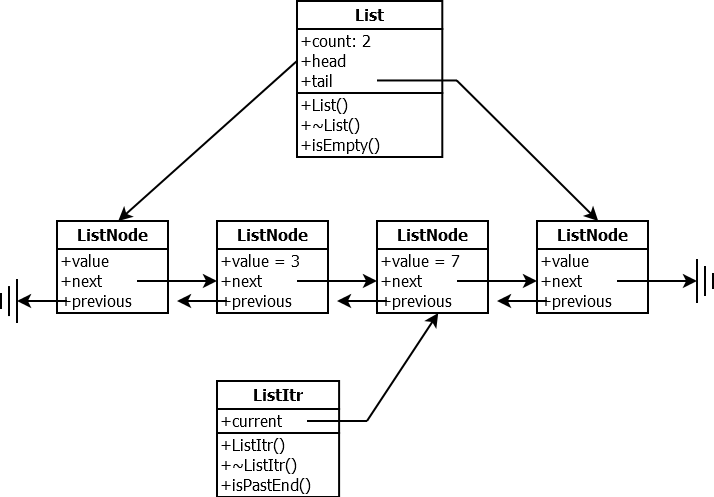
\includegraphics[height=0.9\textheight]{list-diagram}
\end{frame}

\begin{frame}[fragile,label=labListDecl]{the lab's list declaration}
\lstset{
    language=C++,
    style=small,
    moredelim={**[is][\btHL<all:2>]{@2}{2@}},
    moredelim={**[is][\btHL<all:3>]{@3}{3@}},
    moredelim={**[is][\btHL<all:4>]{@4}{4@}},
}
\begin{lstlisting}
class ListNode {

public:
    ListNode();                // Constructor
    ...
private:
    int value;
    @2ListNode *next, *previous2@;

    @3friend class List;3@
    @4friend class ListItr;4@
};
\end{lstlisting}
\begin{tikzpicture}[overlay,remember picture]
\coordinate (place) at ([yshift=4cm]current page.south);
\tikzset{
    markBox/.style={draw=red,very thick,align=left,at=(place), fill=white},
}
\begin{visibleenv}<2>
\node[markBox] {\texttt{*} binds to name --- declares two pointers; \\
                (why I write \texttt{*} next to names)};
\end{visibleenv}
\begin{visibleenv}<3>
\node[markBox] {the class \texttt{List} can access \\ private members of \texttt{ListNode}};
\end{visibleenv}
\begin{visibleenv}<4>
\node[markBox] {the class \texttt{ListItr} can access \\ private members of \texttt{ListNode}};
\end{visibleenv}
\end{tikzpicture}
\end{frame}

\begin{frame}[fragile,label=labListLocal]{a common mistake}
\lstset{
    language=C++,
    style=small,
    moredelim={**[is][\btHL<all:2>]{@2}{2@}},
    moredelim={**[is][\btHL<all:3>]{@3}{3@}},
    moredelim={**[is][\btHL<all:4>]{@4}{4@}},
}
\begin{lstlisting}
class Foo {
public:
  Foo();
private:
  ListNode *@2head2@;
  ...
};
Foo::Foo() {
  ListNode *@2head2@ = new ListNode; // BROKEN!
}
\end{lstlisting}
\begin{itemize}
\item what's wrong with this?
\end{itemize}
\begin{tikzpicture}[overlay,remember picture]
    \tikzset{
        >=Latex,
    }
\coordinate (place) at ([yshift=8cm,xshift=0cm]current page.south);
\begin{visibleenv}<2->
\node[draw,font=\tt,thick,anchor=north west,label={north:Foo object},minimum width=2cm] (fooHead) at (place) {
    head
};
\node[draw,font=\tt,thick,anchor=north west,minimum width=2cm] (fooRest) at (fooHead.south west) {\ldots};
    \node[draw,font=\tt,thick,anchor=north west,label={north:local variables}] (fooLocal) at ([yshift=-2.5cm]place) {
    head
};
\end{visibleenv}
\begin{visibleenv}<3->
    \node[right=1cm of fooHead,label={north:ListNode},rectangle split,rectangle split parts=3,draw] (fooNode) {
    next
    \nodepart{second} prev
    \nodepart{third} \ldots
};
    \draw[ultra thick,red,->] (fooLocal) -- ++(1cm,0cm) |- (fooNode)
\end{visibleenv}
\end{tikzpicture}
\end{frame}


\section{heap implementation}

\begin{frame}{heap example}
\begin{itemize}
\item linked off slides page as
\item \texttt{binary\_heap.h}
\item \texttt{binary\_heap.cpp}
\vspace{.5cm}
\item you may use for lab
\end{itemize}
\end{frame}


\subsection{class declaration, constructor}

% FIXME: emphasize weird constructor
% FIXME:
\begin{frame}[fragile,label=heapPublic]{heap declaration: public}
\lstset{language=C++,style=small}
\begin{lstlisting}
class binary_heap {
public:
    binary_heap();
    binary_heap(vector<int> vec);
    ~binary_heap();
    
    void insert(int x);
    int findMin();
    int deleteMin();
    unsigned int size();
    void makeEmpty();
    bool isEmpty();
    void print();
    ...
};
\end{lstlisting}
\end{frame}

\begin{frame}[fragile,label=heapPrivate]{heap declaration: private}
\lstset{language=C++,style=small}
\begin{lstlisting}
class binary_heap {
    ...
private:
    vector<int> heap;
    unsigned int heap_size;
    void percolateUp(int hole);
    void percolateDown(int hole);
};
\end{lstlisting}
\end{frame}

\begin{frame}[fragile,label=vectorHeap]{vector heap}
\lstset{language=C++,style=small}
\begin{itemize}
\item \lstinline|vector<int> heap| --- vector representing binary tree, using rules shown before
\begin{itemize}
\item \lstinline|heap[0]| is unused
\item \lstinline|heap[1]| is root
\item \lstinline|heap[i * 2]| is left child of node $i$
\item \lstinline|heap[i * 2 + 1]| is right child of node $i$
\end{itemize}
\item \lstinline|int heap_size| is its size 
\begin{itemize}
\item (even though \texttt{heap.size() - 1} could have been used instead\ldots)
\end{itemize}
\end{itemize}
\end{frame}

\begin{frame}[fragile,label=constructFromHeap]{binary\_heap::binary\_heap(vec)} 
\lstset{language=C++,style=small}
\begin{itemize}
\item constructor to initialize from \textit{unsorted} vector
\item equivalent to repeated insertion\ldots
\item<2-> recall: in-place heap sort --- similar to what's happening here\ldots
\end{itemize}
\begin{lstlisting}
binary_heap::binary_heap(vector<int> vec) : 
        heap_size(vec.size()) {
    heap = vec;
    heap.push_back(heap[0]);
    heap[0] = 0;
    for ( int i = heap_size/2; i > 0; i-- )
        percolateDown(i);
}
\end{lstlisting}
\end{frame}

\begin{frame}[fragile,label=heapMinEtc]{findMin/size/etc.}
\lstset{language=C++,style=small}
\begin{lstlisting}
int binary_heap::findMin() {
    if ( heap_size == 0 )
        throw "findMin() called on empty heap";
    return heap[1];
}

unsigned int binary_heap::size() {
    return heap_size;
}

bool binary_heap::isEmpty() {
    return heap_size == 0;
}

void binary_heap::makeEmpty() {
    heap_size = 0;
    heap.resize(1);
}
\end{lstlisting}
\end{frame}

\begin{frame}[fragile,label=heapPrint]{print}
\lstset{language=C++,style=small}
\begin{lstlisting}
void binary_heap::print() {
    cout << "(" << heap[0] << ") ";
    for ( int i = 1; i <= heap_size; i++ ) {
        cout << heap[i] << " ";
        // next line from from http://tinyurl.com/mf9tbgm
        bool isPow2 = (((i+1) & ~(i))==(i+1))? i+1 : 0;
        if ( isPow2 )
            cout << endl << "\t";
    }
    cout << endl;
}
\end{lstlisting}
\end{frame}


% FIXME: missing findMin, etc.

\subsection{print}

% Probably unneeded

\subsection{ASCII}

\subsection{recall: full binary tree}


